
% ----------------------------------------------------------------------
%  Set the document class
% ----------------------------------------------------------------------
\documentclass[11pt,a4paper,twoside]{article}

% ----------------------------------------------------------------------
% Define external packages, language, margins, fonts and new commands
% ----------------------------------------------------------------------
%\input{preamble} 
\usepackage[utf8]{inputenc}   % <<<<< Linux
\usepackage[english]{babel} % <<<<< English
\usepackage{notoccite}
\usepackage[skip=0.5\baselineskip]{caption}
\hyphenation{GTKWave}
\usepackage{listings}
\usepackage[all]{nowidow}
\usepackage[skip=2pt]{caption}
\usepackage{indentfirst}
\newcommand{\squeezeup}{\vspace{-4.5mm}}
%blind text
\usepackage{lipsum}

\usepackage{graphicx}
\graphicspath{ {./} {../../figlib/} }
\def\FontLn{% 16 pt normal
  \usefont{T1}{phv}{m}{n}\fontsize{16pt}{16pt}\selectfont}
\def\FontLb{% 16 pt bold
  \usefont{T1}{phv}{b}{n}\fontsize{16pt}{16pt}\selectfont}
\def\FontMn{% 14 pt normal
  \usefont{T1}{phv}{m}{n}\fontsize{14pt}{14pt}\selectfont}
\def\FontMb{% 14 pt bold
  \usefont{T1}{phv}{b}{n}\fontsize{14pt}{14pt}\selectfont}
\def\FontSn{% 12 pt normal
  \usefont{T1}{phv}{m}{n}\fontsize{12pt}{12pt}\selectfont}

% Use Arial font as default
%
\renewcommand{\rmdefault}{phv}
\renewcommand{\sfdefault}{phv}
\usepackage{geometry}	
\geometry{verbose,tmargin=2.5cm,bmargin=2.5cm,lmargin=2.5cm,rmargin=2.5cm}

%\usepackage{setspace}
%\renewcommand{\baselinestretch}{1.5}

\usepackage[pdftex]{hyperref} % enhance documents that are to be
                              % output as HTML and PDF
\hypersetup{colorlinks,       % color text of links and anchors,
                              % eliminates borders around links
%            linkcolor=red,    % color for normal internal links
            linkcolor=black,  % color for normal internal links
            anchorcolor=black,% color for anchor text
%            citecolor=green,  % color for bibliographical citations
            citecolor=black,  % color for bibliographical citations
%            filecolor=magenta,% color for URLs which open local files
            filecolor=black,  % color for URLs which open local files
%            menucolor=red,    % color for Acrobat menu items
            menucolor=black,  % color for Acrobat menu items
%            pagecolor=red,    % color for links to other pages
            pagecolor=black,  % color for links to other pages
%            urlcolor=cyan,    % color for linked URLs
            urlcolor=black,   % color for linked URLs
	          bookmarks=true,         % create PDF bookmarks
	          bookmarksopen=false,    % don't expand bookmarks
	          bookmarksnumbered=true, % number bookmarks
	          pdftitle={report},
            pdfauthor={Andre C. Marta},
%            pdfsubject={Thesis Title},
%            pdfkeywords={Thesis Keywords},
            pdfstartview=FitV,
            pdfdisplaydoctitle=true}

\usepackage[numbers,sort&compress]{natbib} % <<<<< References in numbered list [1],[2],...
\usepackage{subcaption} 
\usepackage{mdframed}

%%%%%%%%%%%%%%%%%%%%%%%%%%%%%%%%%%%%%%%%%%%%%%%%%%%%%%%%%%%%%%%%%%%%%%%%
%     Begin Document                                                   %
%%%%%%%%%%%%%%%%%%%%%%%%%%%%%%%%%%%%%%%%%%%%%%%%%%%%%%%%%%%%%%%%%%%%%%%%


\begin{document}

% Set plain page style (no headers, footer with centered page number)
\pagestyle{plain}

% Set roman numbering (i,ii,...) before the start of chapters
%\pagenumbering{roman}

% ----------------------------------------------------------------------
%  Cover page
% ----------------------------------------------------------------------
%%%%%%%%%%%%%%%%%%%%%%%%%%%%%%%%%%%%%%%%%%%%%%%%%%%%%%%%%%%%%%%%%%%%%%%%
%                                                                      %
%     File: Thesis_FrontCover.tex                                      %
%     Tex Master: Thesis.tex                                           %
%                                                                      %
%     Author: Andre C. Marta                                           %
%     Last modified :  2 Jul 2015                                      %
%                                                                      %
%%%%%%%%%%%%%%%%%%%%%%%%%%%%%%%%%%%%%%%%%%%%%%%%%%%%%%%%%%%%%%%%%%%%%%%%

\thispagestyle {empty}

% IST Logo - Signature A
% parameters: bb=llx lly urx ury (bounding box), width=h_length, height=v_length, angle=angle, scale=factor, clip=true/false, draft=true/false. 
\includegraphics[bb=9.5cm 11cm 0cm 0cm,scale=0.29]{IST_A_CMYK_POS}

\begin{center}
%
% Figure (Image or plot)
\vspace{1.0cm}
% height = 50 mm
%\includegraphics[height=50mm]{Figures/Airbus_A350.jpg}

% Title, author and degree
\vspace{1cm}
{\FontLb Circuit Theory and Electronics Fundamentals} \\ % <<<<< EDIT TITLE
\vspace{1cm}
{\FontSn Department of Electrical and Computer Engineering, Técnico, University of Lisbon} \\ % <<<<< EDIT COURSE
\vspace{1cm}
{\FontSn Example Laboratory Report} \\
\vspace{1cm}
{\FontSn February 27, 2021} \\ % <<<<< EDIT DATE (corresponds to date of oral examination)
%
\end{center}



% ----------------------------------------------------------------------
% Dedication page (optional)
% ----------------------------------------------------------------------
%\input{dedication} 
%\cleardoublepage

% ----------------------------------------------------------------------
%  Acknowledgments (optional)
% ----------------------------------------------------------------------
%\input{acknowledgements}
%\cleardoublepage

% ----------------------------------------------------------------------
%  Abstract (both in English and Portuguese)
% ----------------------------------------------------------------------
%\input{resumo} 
%\cleardoublepage

%\input{abstract} 

% ----------------------------------------------------------------------
%  Table of contents, list of tables, list of figures and nomenclature
% ----------------------------------------------------------------------

% Table of contents
%
\tableofcontents

% List of tables
%\addcontentsline{toc}{section}{\listtablename}
%\listoftables
%\cleardoublepage 

% List of figures
%\addcontentsline{toc}{section}{\listfigurename}
%\listoffigures
%\cleardoublepage 

% Set arabic numbering (1,2,...) after preface
%
%\setcounter{page}{1}
%\pagenumbering{arabic}

% ----------------------------------------------------------------------
%  Body
% ----------------------------------------------------------------------

\newpage
\section{Introduction}
\label{sec:introduction}

% state the learning objective 

The objective of this laboratory assignment is to do analysis on a circuit using the mesh and the nodal method as well as running a simulation using NgSpice with the objective of detecting small diferences between the different approcahes and understand why said differences happen. The circuit can be seen in Figure~\ref{fig:rc}.

In Section~\ref{sec:analysis}, a theoretical analysis of the circuit is
presented. In Section~\ref{sec:simulation}, the circuit is analysed by
simulation, and the results are compared to the theoretical results obtained in
Section~\ref{sec:analysis}. The conclusions of this study are outlined in
Section~\ref{sec:conclusion}.

\squeezeup
\begin{figure}[h!] \centering
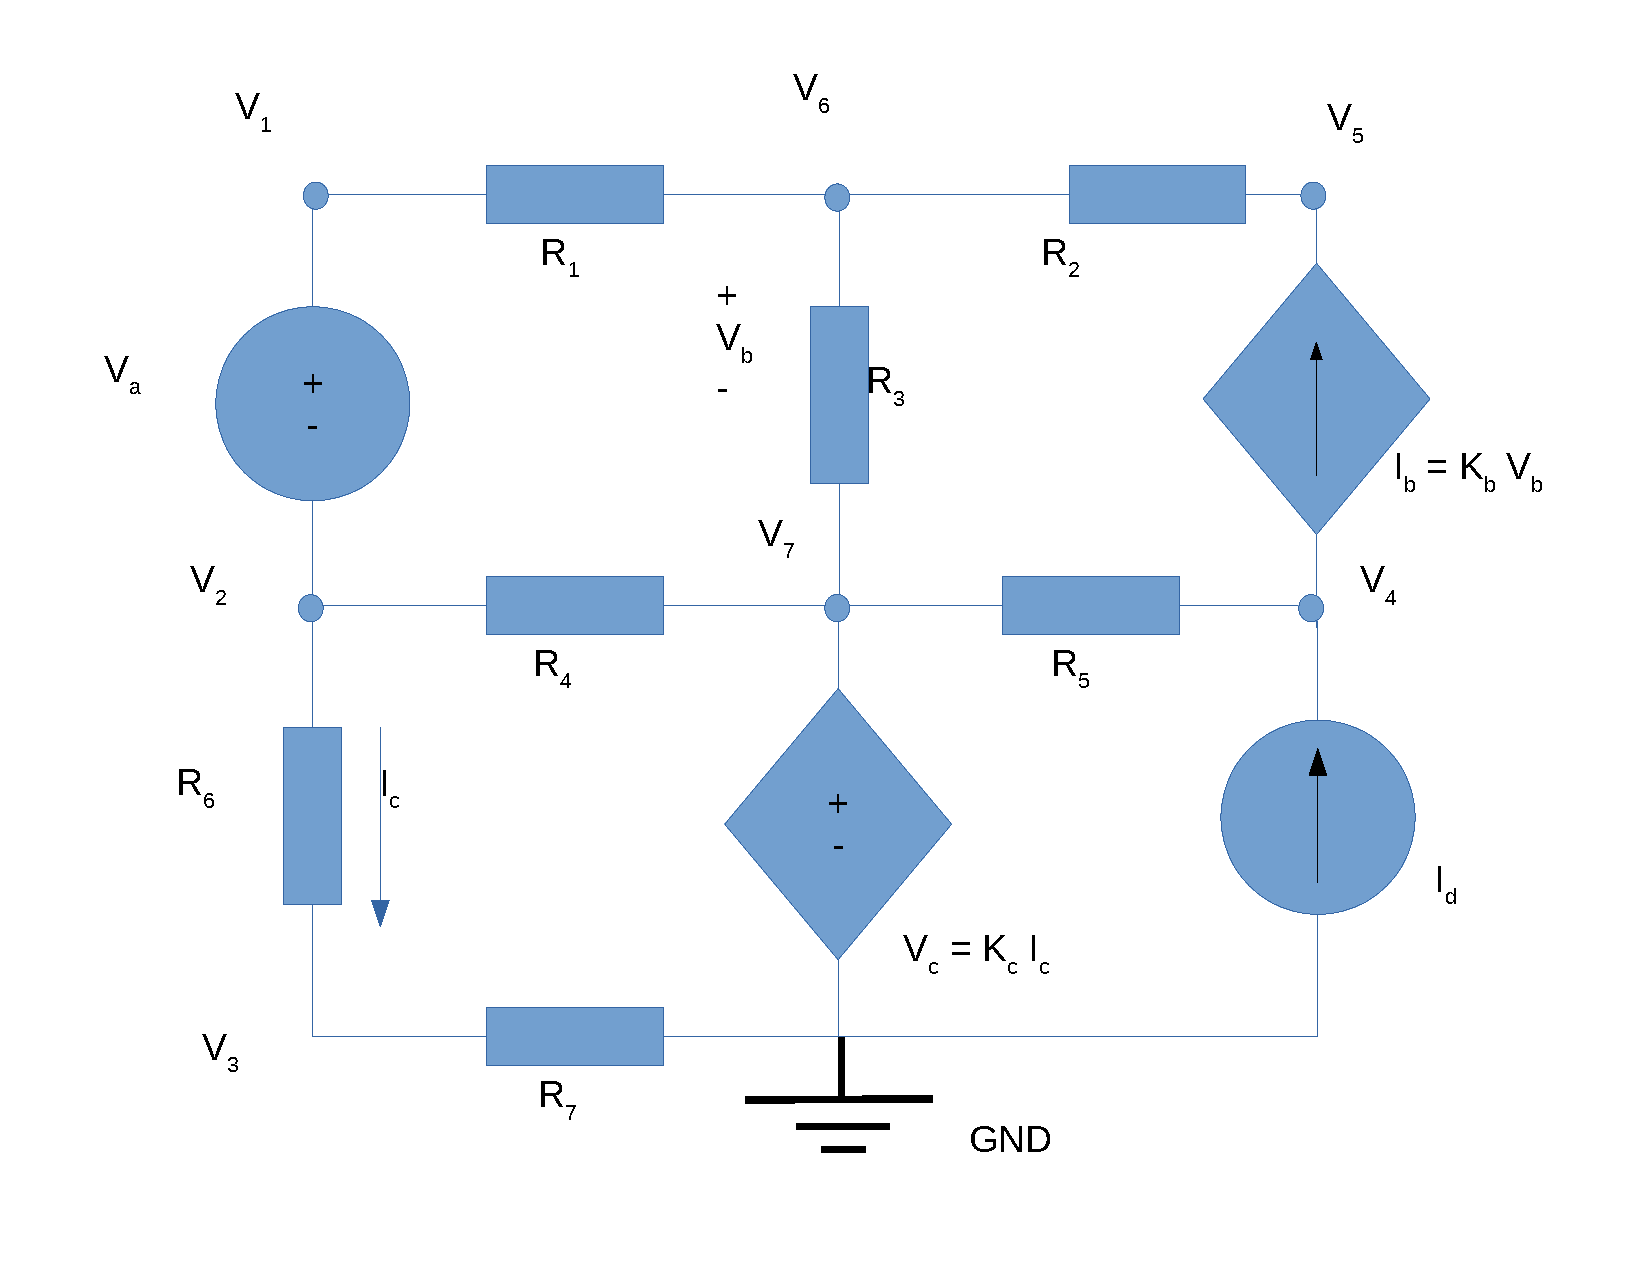
\includegraphics[width=0.8\textwidth, scale=1.0]{rc.pdf}
\squeezeup
\caption{Circuit with an independent current and voltage source ($V_a$ and $I_d$ respectively) and linear dependent sources ($V_c$-linear current controlled voltage source and $I_b$-linear voltage controlled current source}
\label{fig:rc}
\end{figure}

The values given for this report can be found in table~\ref{tab:op1}.

\begin{table}[hb]
  \centering
  \begin{tabular}{|l|r|}
    \hline    
    {\bf Name} & {\bf Values} \\ \hline
    R1 & 1.01949191994 Kohms\\ \hline
R2 & 2.05054429461 Kohms\\ \hline
R3 & 3.09286027724 Kohms\\ \hline
R4 & 4.12838973576 Kohms\\ \hline
R5 & 3.06635427647 Kohms\\ \hline
R6 & 2.01254230153 Kohms\\ \hline
R7 & 1.00502981701 Kohms\\ \hline
Va & 5.24204797361 V\\ \hline
Id & 1.01905568201 mA\\ \hline
Kb & 7.23185131759 mS\\ \hline
Kc & 8.12820254987 Kohms\\ \hline

  \end{tabular}
  \caption{Values received by the Python program.}
  \label{tab:op1}
\end{table}




\newpage
\section{Theoretical Analysis}
\label{sec:analysis}

\subsection{Mesh Analysis}
\begin{figure}[h] \centering
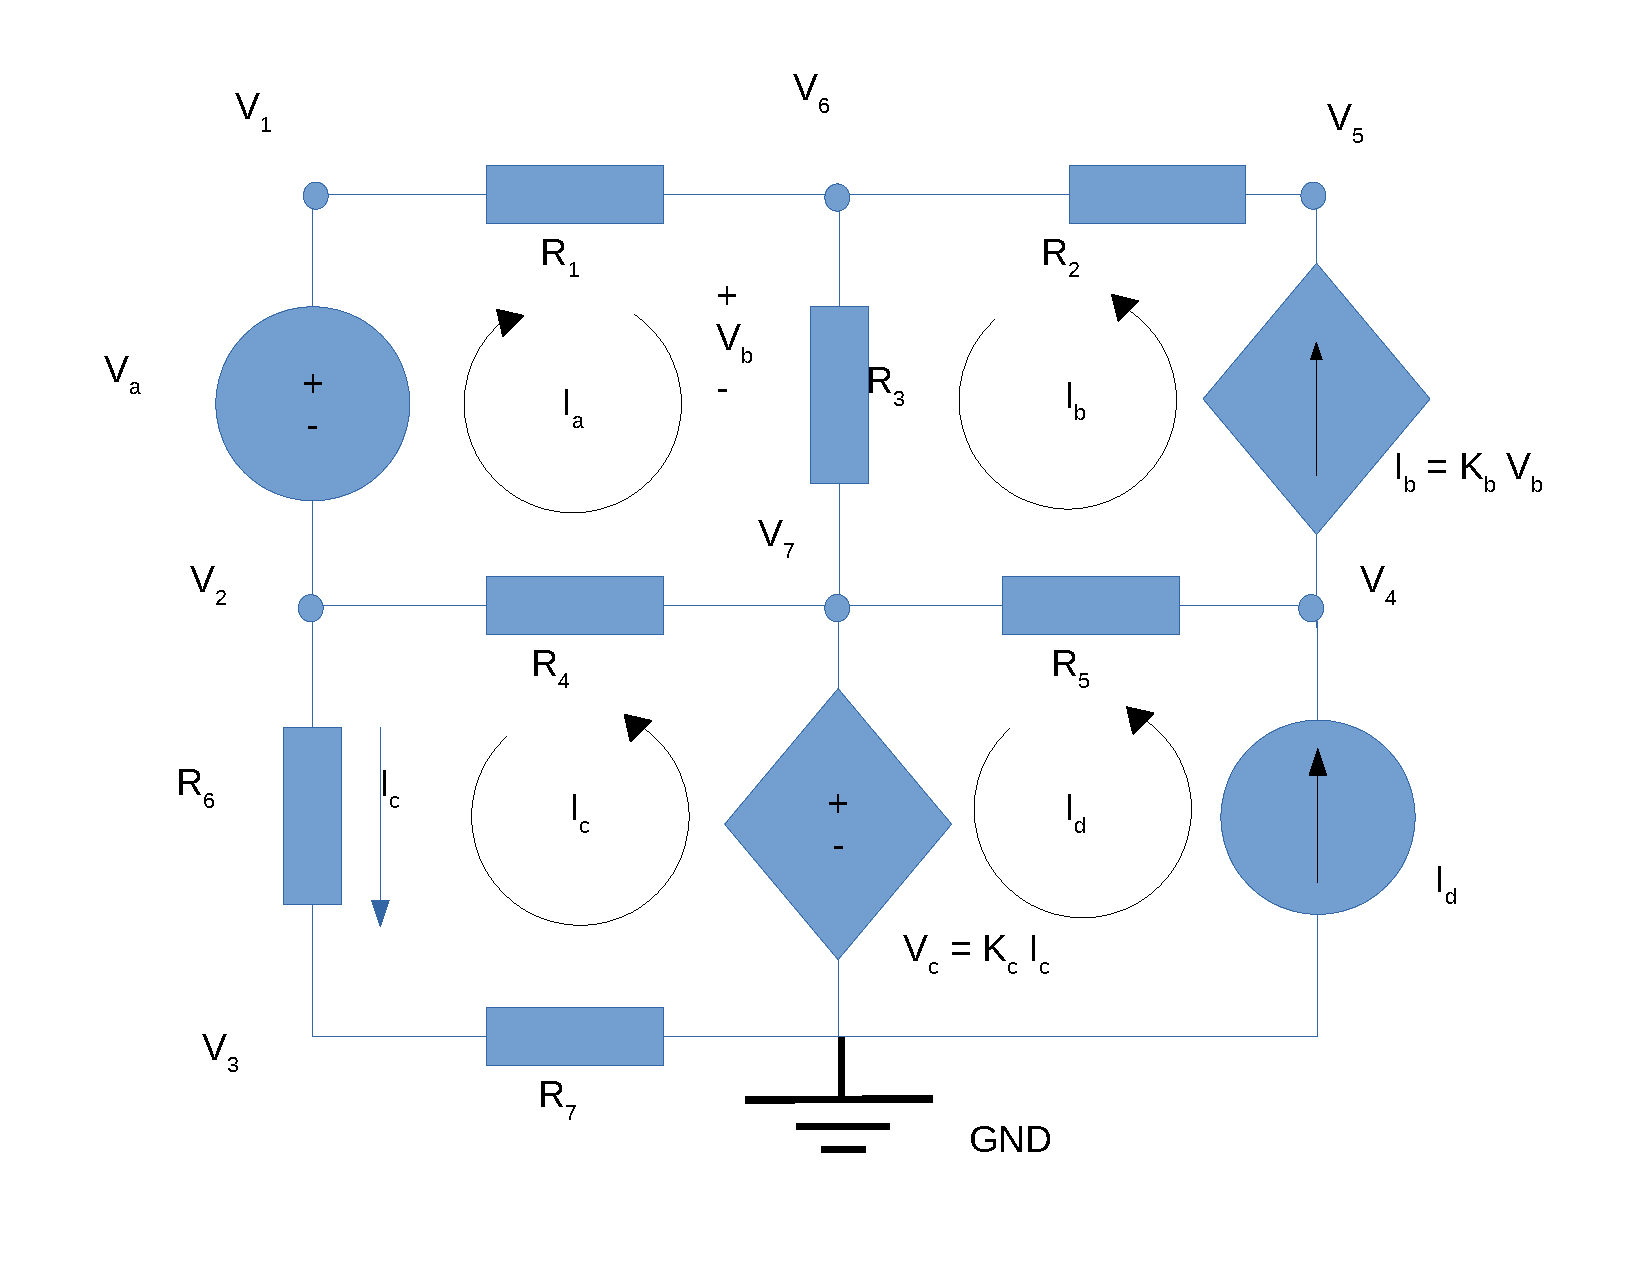
\includegraphics[width=0.8\linewidth]{rc1.pdf}
\caption{Representation of mesh currents in the circuit.}
\label{fig:meshcurrents}
\end{figure}

Figure~\ref{fig:meshcurrents} shows the mesh currents considered for the circuit analysis, with the current $I_a$ flowing clockwise and the rest of the currents ($I_b$, $I_c$ and $I_d$) flowing counter-clockwise. In the meshes containing $I_b$ and $I_d$, the currents were considered to be the same as the current sources in said meshes.

From this circuit, there can then be extracted 3 equations to figure out the value of the components necessary for the circuit analysis.

The first one, Equation~\ref{eq:meshb} , was obtained by using Ohm's Law, assuming it is known the value of the voltage and the resistence in resistor 3 and that the current flowing through it is ($I_a$ + $I_b$).
\begin{equation}
  I_{b} = K_{b}(I_{a} + I_{b})R_{3},
  \label{eq:meshb}
\end{equation}

Equation~\ref{eq:mesha}  was figured out by analysing the top left mesh, using Kirchoff's Voltage Law and Ohm's Law for the resistors. Since the current $I_a$ is flowing clockwise, the voltage in $V_a$ is negative and the currents in resistors 3 and 4 are, 
correspondingly, ($I_a$ + $I_b$) and ($I_a$ + $I_c$), as these pairs of currents are flowing the same way in said resistors.
\begin{equation}
  -V_{a} + I_{a}R_{1} + (I_{a} + I_{b})R_{3} + (I_{a} + I_{c})R_{4} = 0,
  \label{eq:mesha}
\end{equation}

Finally, from the bottom left mesh, there is Equation~\ref{eq:meshc}, in which was also used Kirchoff's Voltage Law and Ohm's Law. The voltage in $V_ac$ is negative due to the current flow.
\begin{equation}
  -K_{c}I_{c} + I_{c}R_{6} + I_{c}R_{7} + (I_{a} + I_{c})R_{4} = 0,
  \label{eq:meshc}
\end{equation}

By developing these 3 equations, the matrix below (\ref{eq:matrix}) is achieved as to simplify the calculations. This matrix was solved in Octave, getting the values of the currents $I_a$, $I_b$ and $I_c$. It was not necessary to solve for the value of the current in the bottom right mesh since it is already known (equivalent to $I_d$).
\begin{equation}
\left[ \begin{array}{ccc} -K_bR_3 & 1-K_bR_3 & 0 \\ R_1+R_3+R_4 & R_3 & R_4 \\ R_4 & 0 & R_6+R_7-K_c+R_4 \end{array} \right]
\times \left[ \begin{array}{c} I_a \\ I_b \\ I_c \end{array} \right] =
\left[ \begin{array}{c} 0 \\ V_a \\ 0 \end{array} \right]
\label{eq:matrix}
\end{equation}

The values of $I_a$, $I_b$ and $I_c$ are then, correspondingly, (2.5852e-4)V, (-2.7062e-4)V and (1.0865e-3)V. With these currents, it is possible to discover the values of the voltages in each node, using the equations~\ref{eq:node7} through~\ref{eq:node1} down below and knowing that $I_b$ = $K_b$$V_b$ and $V_c$=$K_c$$I_c$.
\begin{equation}
  V_{7} = V_{c},
  \label{eq:node7}
\end{equation}

\begin{equation}
  V_{6} = V_{7} + V_{b},
  \label{eq:node6}
\end{equation}

\begin{equation}
  V_{5} = V_{6} + R_{2}I_{b},
  \label{eq:node5}
\end{equation}

\begin{equation}
  V_{4} = V_{7} + R_{5}I_{d},
  \label{eq:node4}
\end{equation}

\begin{equation}
  V_{3} = V_{0} + R_{7}I_{c},
  \label{eq:node3}
\end{equation}

\begin{equation}
  V_{2} = V_{3} + R_{6}I_{c},
  \label{eq:node2}
\end{equation}

\begin{equation}
  V_{1} = V_{2} + V_{a},
  \label{eq:node1}
\end{equation}

The following table (\ref{table:nodesmesh}) shows the node voltages discored by replacing the variables with the known values. Notice that the values are not equal to the ones obtained by the simulation analysis or the node analysis. This is due to the fact that the mesh analysis is not as exact as the other methods; however, the results are similar enough to be relevant to this experiment.
\begin{table}[h!]
\centering
\begin{tabular}{ |c|c| } 
 \hline
 {\bf Node} & {\bf Voltage[V]} \\ 
 \hline\hline
 $V_1$ & 8.5206e00 \\ 
 \hline
 $V_2$ & 3.2785e00 \\ 
 \hline
 $V_3$ & 1.0920e00 \\ 
 \hline
 $V_4$ & 1.1956e01 \\ 
 \hline
 $V_5$ & 7.4396e00 \\ 
 \hline
 $V_6$ & 7.9946e00 \\ 
 \hline
 $V_7$ & 8.8313e00 \\ 
 \hline
\end{tabular}
\caption{Voltage values using the mesh analysis.}
\label{table:nodesmesh}
\end{table}

\subsection{Nodal Analysis}


\section{Simulation Analysis}
\label{sec:simulation}

\subsection{Operating Point Analysis}

Table~\ref{tab:op} shows the simulated operating point results for the circuit
under analysis. Compared to the theoretical analysis results, one notices the
following differences: describe and explain the differences.

\begin{table}[h]
  \centering
  \begin{tabular}{|l|r|}
    \hline    
    {\bf Name} & {\bf Value [A or V]} \\ \hline
    @cb[i] & 0.000000e+00\\ \hline
@ce[i] & 0.000000e+00\\ \hline
@q1[ib] & 7.022567e-05\\ \hline
@q1[ic] & 1.404513e-02\\ \hline
@q1[ie] & -1.41154e-02\\ \hline
@q1[is] & 5.765392e-12\\ \hline
@rc[i] & 1.411536e-02\\ \hline
@re[i] & 1.411536e-02\\ \hline
@rf[i] & 7.022567e-05\\ \hline
@rs[i] & 0.000000e+00\\ \hline
v(1) & 0.000000e+00\\ \hline
v(2) & 0.000000e+00\\ \hline
base & 2.254108e+00\\ \hline
coll & 5.765392e+00\\ \hline
emit & 1.411536e+00\\ \hline
vcc & 1.000000e+01\\ \hline

  \end{tabular}
  \caption{Operating point. A variable preceded by @ is of type {\em current}
    and expressed in Ampere; other variables are of type {\it voltage} and expressed in
    Volt.}
  \label{tab:op}
\end{table}

\lipsum[1-1]


\subsection{Transient Analysis}

Figure~\ref{fig:trans} shows the simulated transient analysis results for the
circuit under analysis. Compared to the theoretical analysis results, one
notices the following differences: describe and explain the differences.

\begin{figure}[h] \centering
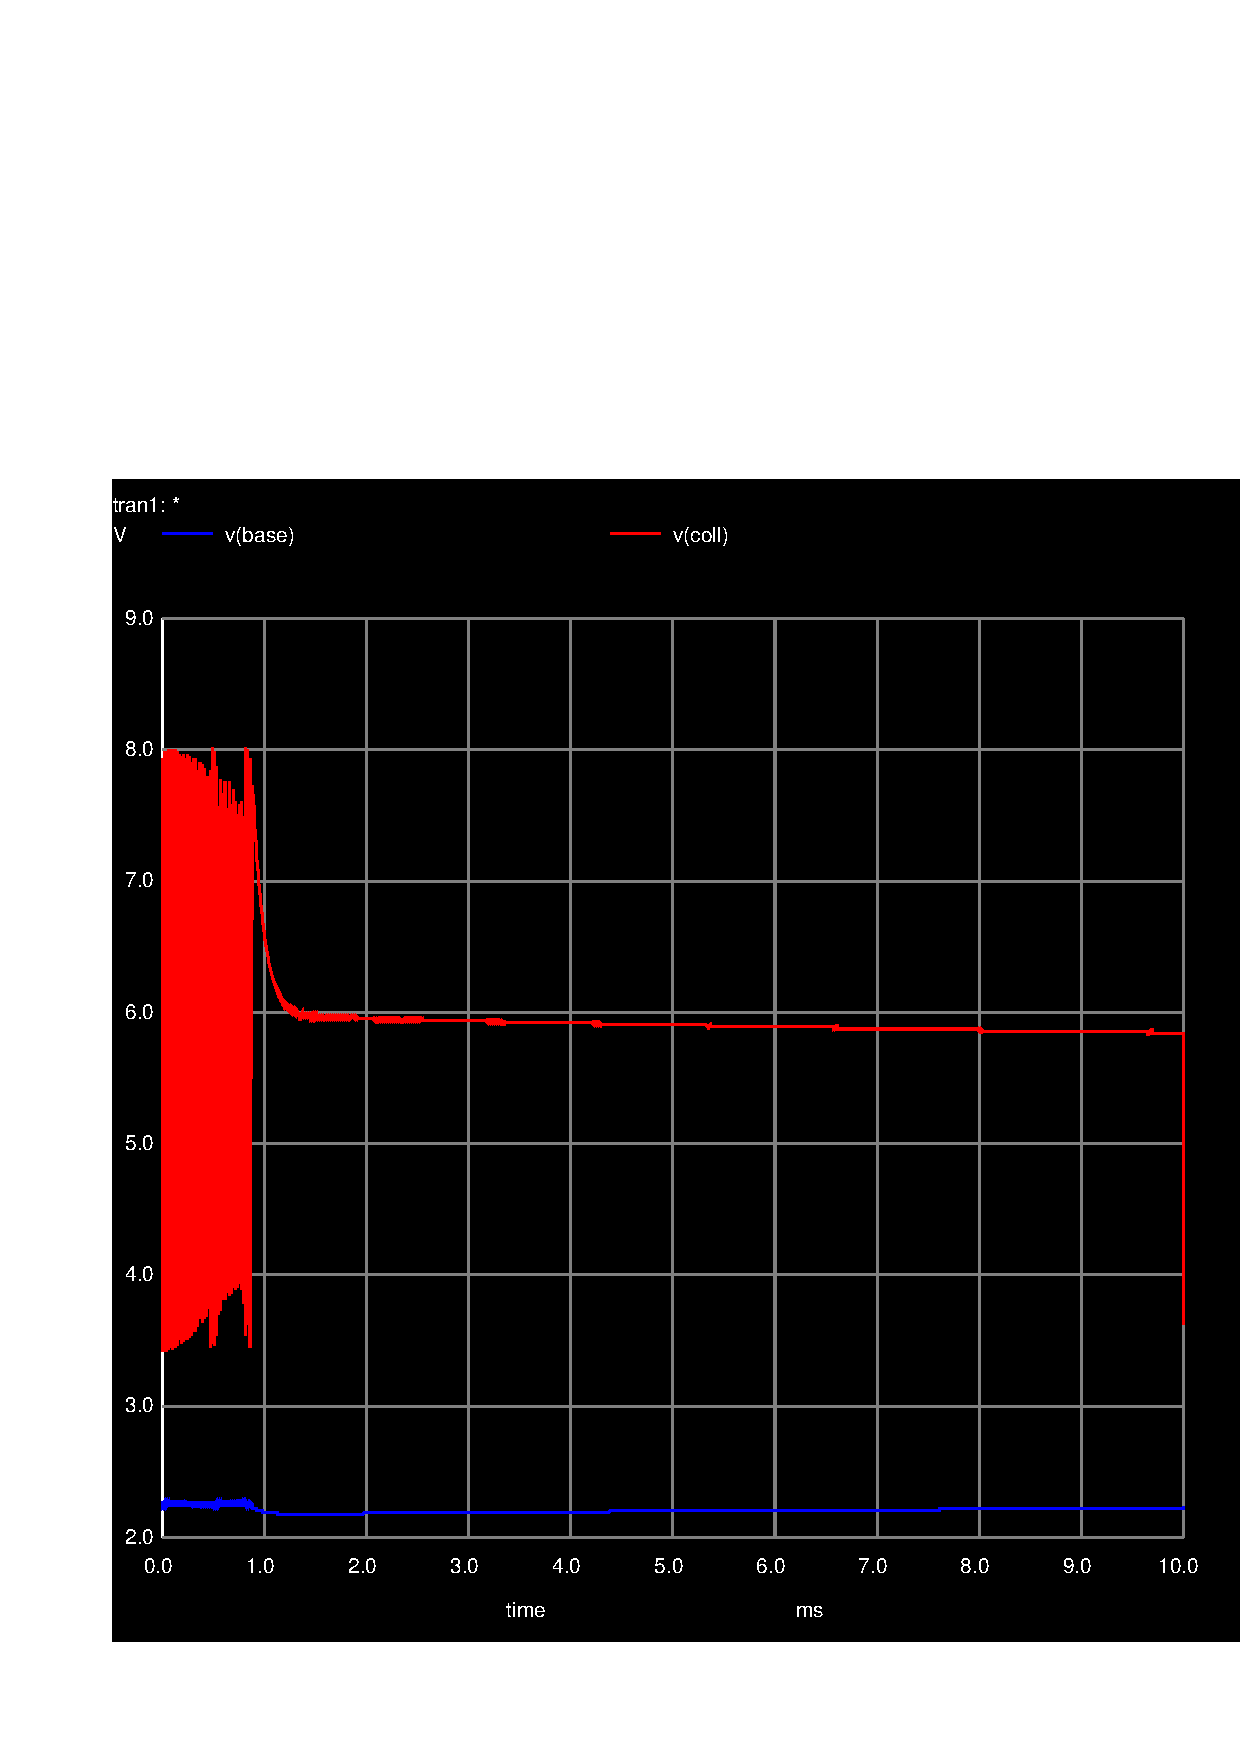
\includegraphics[width=0.6\linewidth]{trans.pdf}
\caption{Transient output voltage}
\label{fig:trans}
\end{figure}

\lipsum[1-1]



\subsection{Frequency Analysis}

\subsubsection{Magnitude Response}

Figure~\ref{fig:acm} shows the magnitude of the frequency response for the
circuit under analysis. Compared to the theoretical analysis results, one
notices the following differences: describe and explain the differences.

\begin{figure}[h] \centering
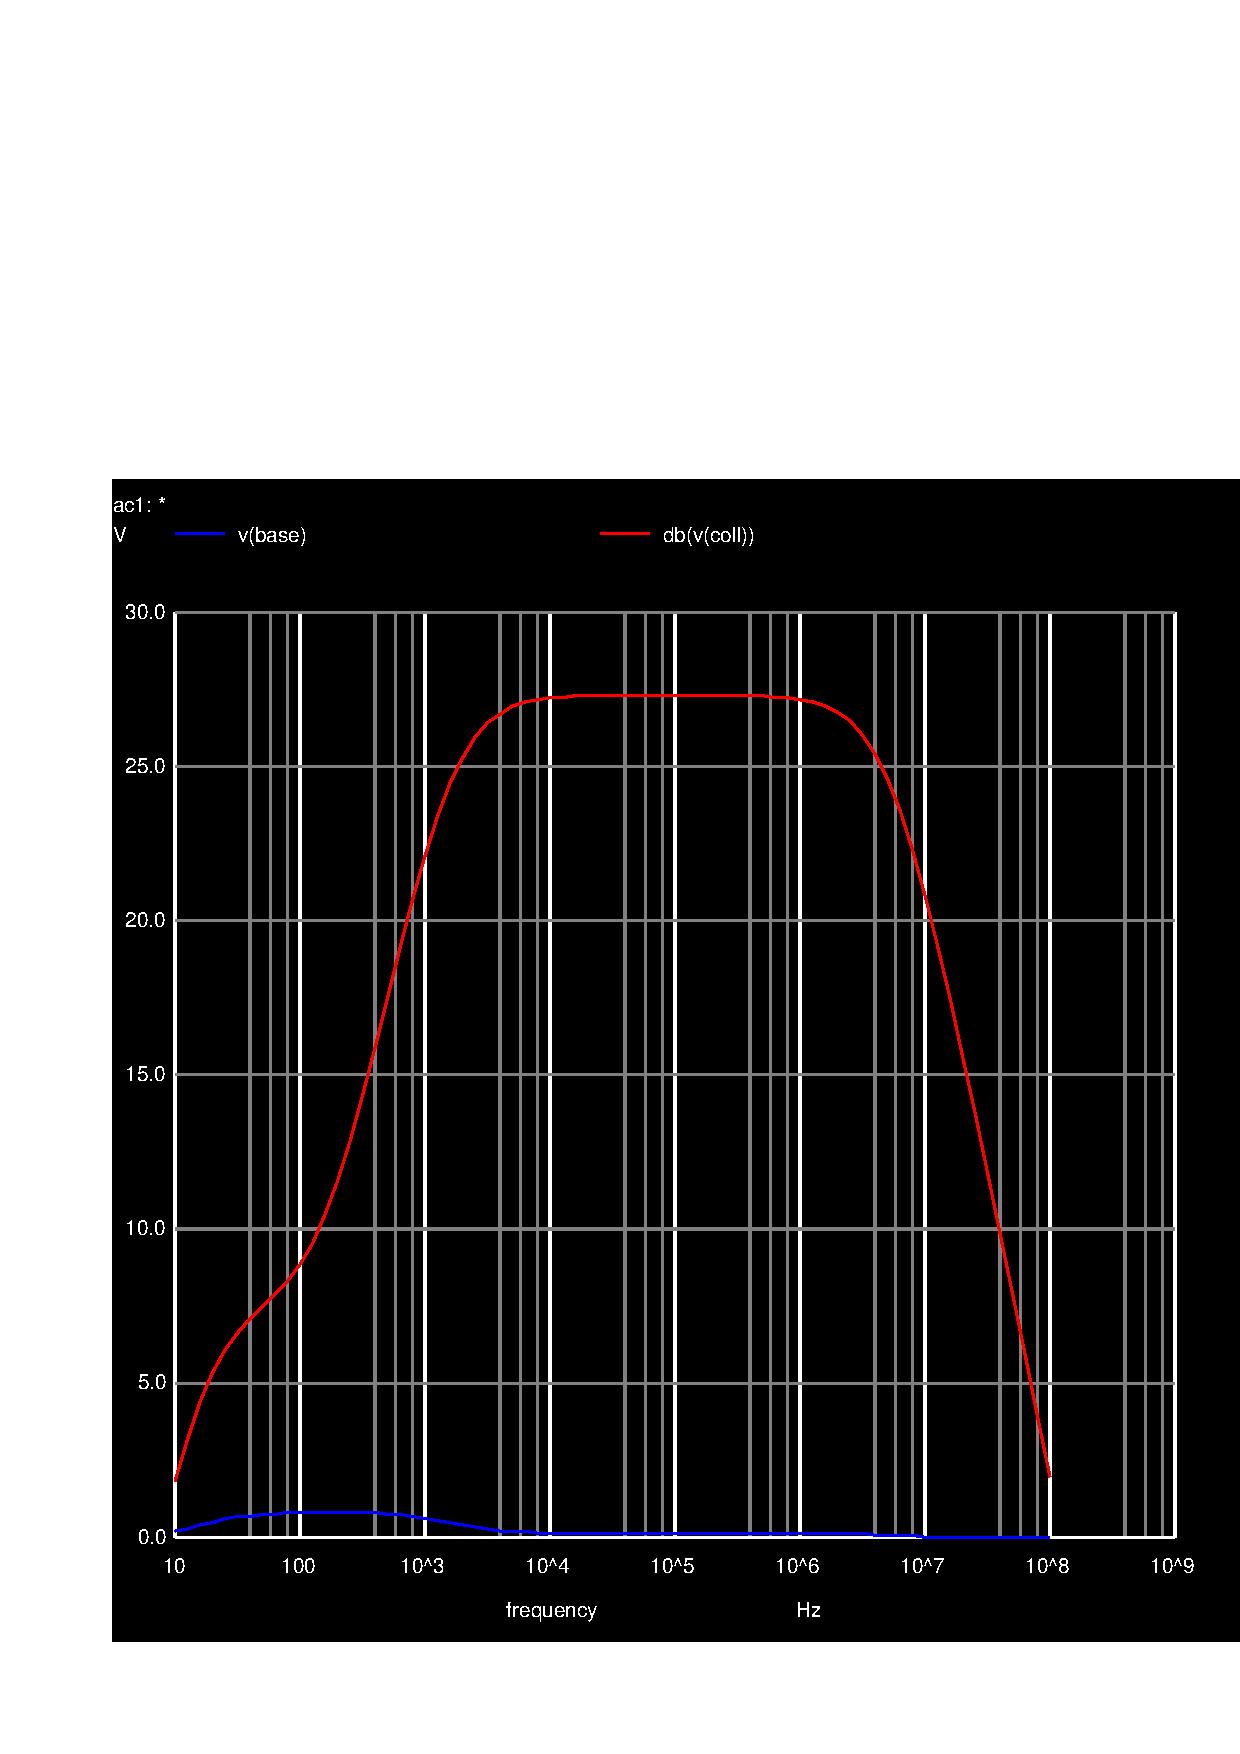
\includegraphics[width=0.6\linewidth]{acm.pdf}
\caption{Magnitude response}
\label{fig:acm}
\end{figure}

\lipsum[1-1]

\subsubsection{Phase Response}

Figure~\ref{fig:acp} shows the magnitude of the frequency response for the
circuit under analysis. Compared to the theoretical analysis results, one
notices the following differences: describe and explain the differences.

\begin{figure}[h] \centering
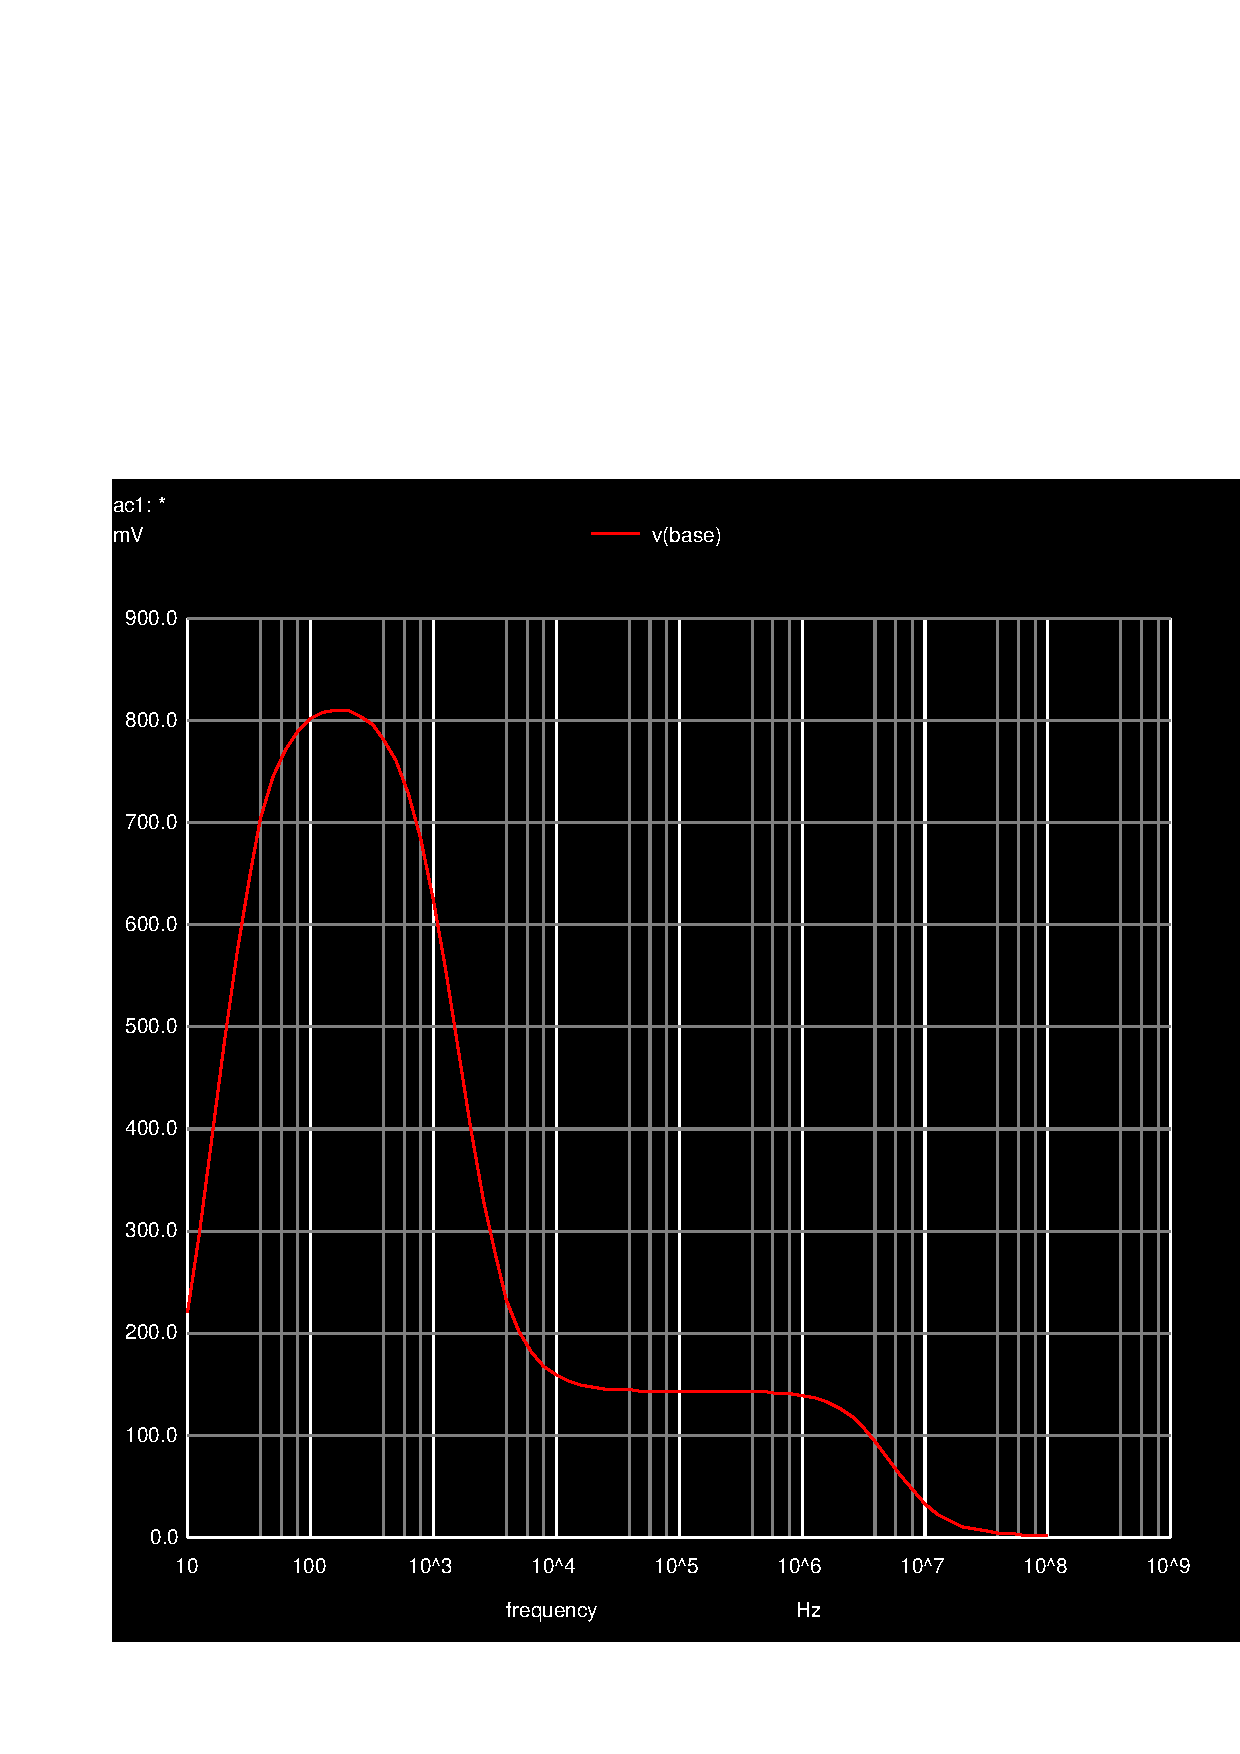
\includegraphics[width=0.6\linewidth]{acp.pdf}
\caption{Phase response}
\label{fig:acp}
\end{figure}

\lipsum[1-1]

\subsubsection{Input Impedance}

Figure~\ref{fig:zim} shows the magnitude of the frequency response for the
circuit under analysis. Compared to the theoretical analysis results, one
notices the following differences: describe and explain the differences.

\begin{figure}[h] \centering
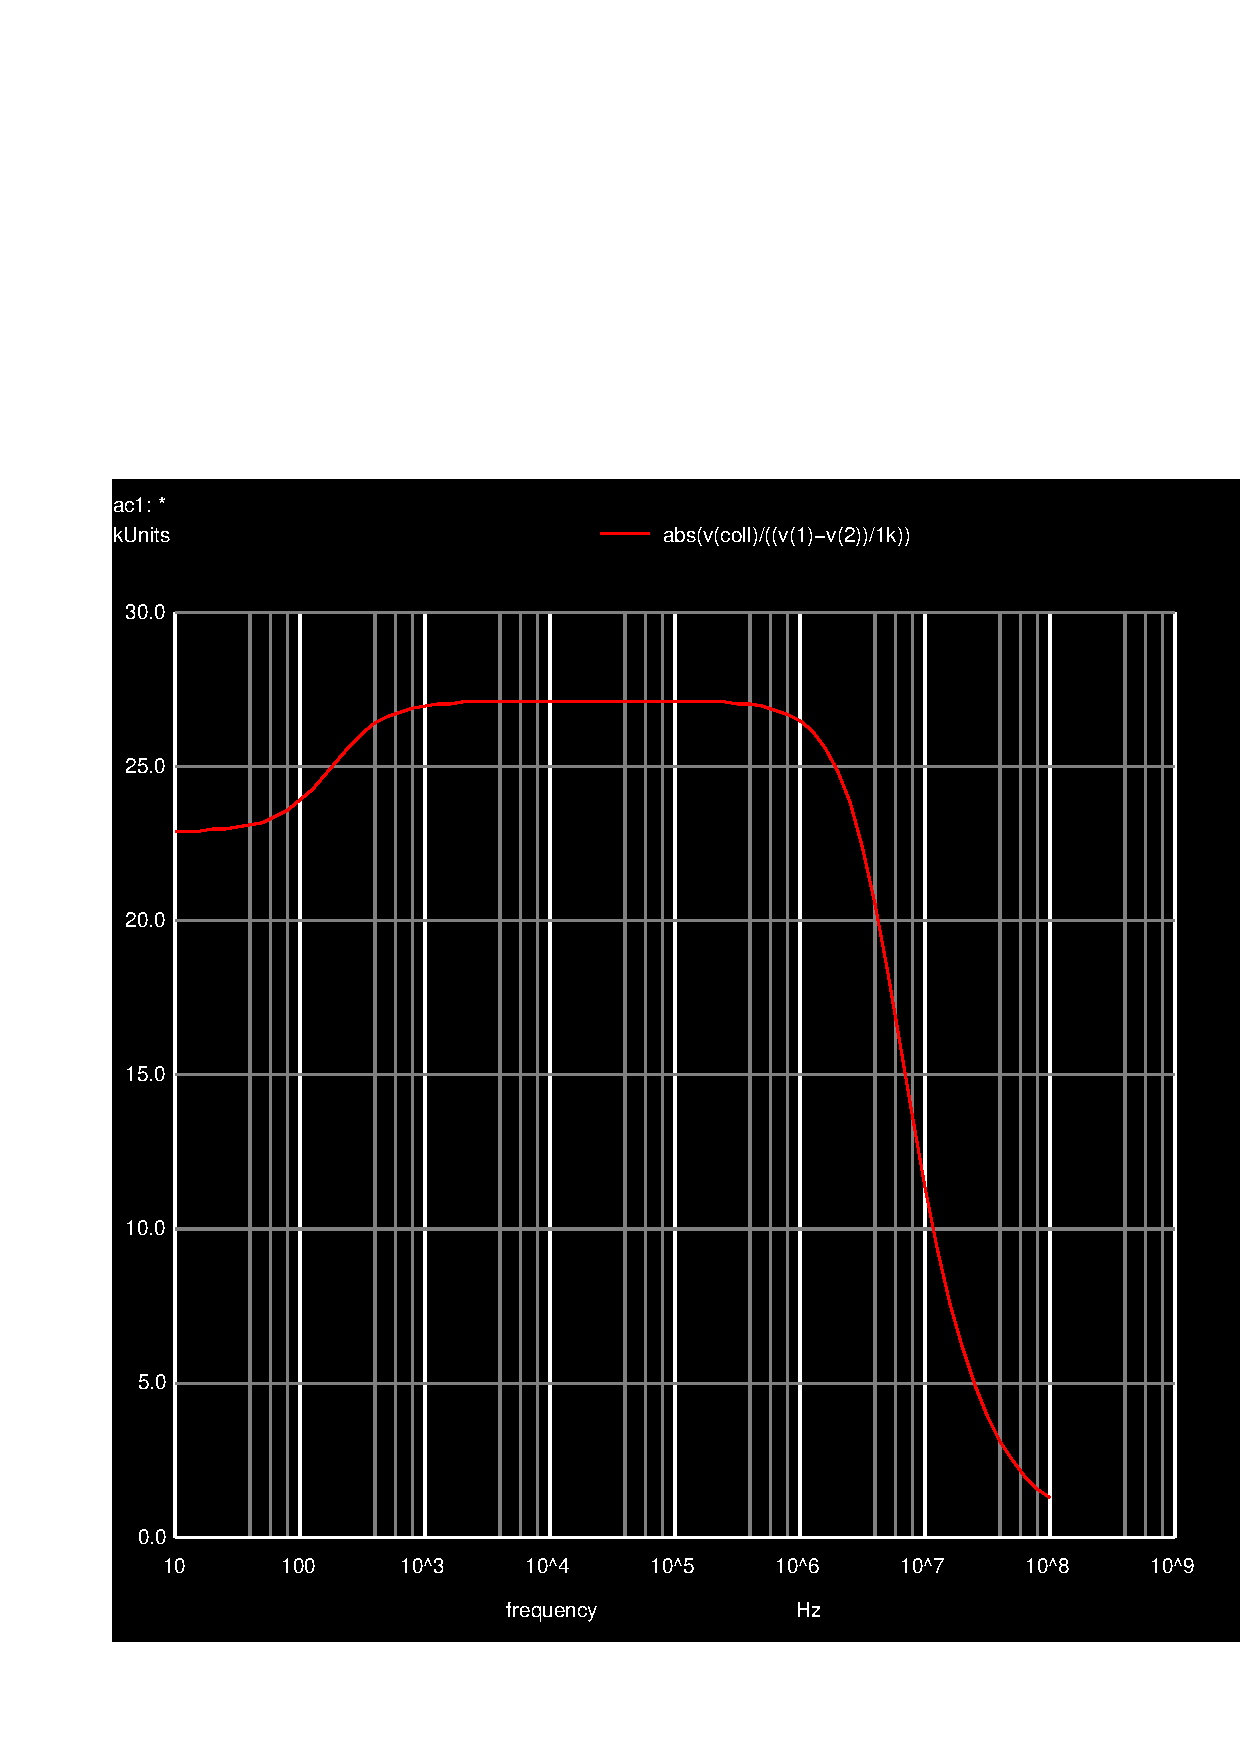
\includegraphics[width=0.6\linewidth]{zim.pdf}
\caption{Input impedance}
\label{fig:zim}
\end{figure}

\lipsum[1-1]





\newpage
\section{Conclusion}
\label{sec:conclusion}

TO BE DONE



%\cleardoublepage

% ----------------------------------------------------------------------
%  Bibliography
% ----------------------------------------------------------------------
%\addcontentsline{toc}{section}{\bibname}
%\bibliographystyle{abbrvunsrtnat} % <<<<< SELECT IF USING REFERENCES BY NUMBER (CITATION ORDER)
%\bibliography{../../../BIBfile.bib}

% ----------------------------------------------------------------------
\end{document}
% ----------------------------------------------------------------------

